%%
%% This is file `sigconf.tex',
%% generated with the docstrip utility.
%%
%% The original source files were:
%%
%% samples.dtx  (with options: `all,proceedings,sigconf')
%% 
%% IMPORTANT NOTICE:
%% 
%% For the copyright see the source file.
%% 
%% Any modified versions of this file must be renamed
%% with new filenames distinct from sigconf.tex.
%% 
%% For distribution of the original source see the terms
%% for copying and modification in the file samples.dtx.
%% 
%% This generated file may be distributed as long as the
%% original source files, as listed above, are part of the
%% same distribution. (The sources need not necessarily be
%% in the same archive or directory.)
%%
%%
%% Commands for TeXCount
%TC:macro \cite [option:text,text]
%TC:macro \citep [option:text,text]
%TC:macro \citet [option:text,text]
%TC:envir table 0 1
%TC:envir table* 0 1
%TC:envir tabular [ignore] word
%TC:envir displaymath 0 word
%TC:envir math 0 word
%TC:envir comment 0 0
%%
%% The first command in your LaTeX source must be the \documentclass
%% command.
%%
%% For submission and review of your manuscript please change the
%% command to \documentclass[manuscript, screen, review]{acmart}.
%%
%% When submitting camera ready or to TAPS, please change the command
%% to \documentclass[sigconf]{acmart} or whichever template is required
%% for your publication.
%%
%%
\documentclass[sigconf]{acmart}
\microtypesetup{expansion=false}
%%
%% \BibTeX command to typeset BibTeX logo in the docs
\AtBeginDocument{%
  \providecommand\BibTeX{{%
    Bib\TeX}}}

%% Rights management information.  This information is sent to you
%% when you complete the rights form.  These commands have SAMPLE
%% values in them; it is your responsibility as an author to replace
%% the commands and values with those provided to you when you
%% complete the rights form.
\setcopyright{acmlicensed}
\copyrightyear{2026}
\acmYear{2026}
\acmDOI{XXXXXXX.XXXXXXX}
%% These commands are for a PROCEEDINGS abstract or paper.
\acmConference[Conference acronym 'XX]{Make sure to enter the correct
  conference title from your rights confirmation email}{June 03--05,
  2018}{Woodstock, NY}
%%
%%  Uncomment \acmBooktitle if the title of the proceedings is different
%%  from ``Proceedings of ...''!
%%
%%\acmBooktitle{Woodstock '18: ACM Symposium on Neural Gaze Detection,
%%  June 03--05, 2018, Woodstock, NY}
\acmISBN{978-1-4503-XXXX-X/2018/06}


%%
%% Submission ID.
%% Use this when submitting an article to a sponsored event. You'll
%% receive a unique submission ID from the organizers
%% of the event, and this ID should be used as the parameter to this command.
%%\acmSubmissionID{123-A56-BU3}

%%
%% end of the preamble, start of the body of the document source.
\begin{document}

%%
%% The "title" command has an optional parameter,
%% allowing the author to define a "short title" to be used in page headers.
\title{Evaluation Strategies for Program Slicing in Automated Program Repair}

%%
%% The "author" command and its associated commands are used to define
%% the authors and their affiliations.
\author{Akash Silas Nesakumar}
\email{akashsilas1@gmail.com}
\affiliation{%
  \institution{University of Hildesheim}
  \city{Hildesheim}
  \country{Germany}
}

\author{Son Thien Nguyen}
\email{sonthien225@gmail.com}
\affiliation{%
  \institution{University of Hildesheim}
  \city{Hildesheim}
  \country{Germany}
}

\author{Avnish Raut}
\email{avnishjraut@gmail.com}
\affiliation{%
  \institution{University of Hildesheim}
  \city{Hildesheim}
  \country{Germany}
}

%%
%% By default, the full list of authors will be used in the page
%% headers. Often, this list is too long, and will overlap
%% other information printed in the page headers. This command allows
%% the author to define a more concise list
%% of authors' names for this purpose.
\renewcommand{\shortauthors}{Nesakumar, Nguyen, and Raut}

%%
%% The abstract is a short summary of the work to be presented in the
%% article.
\begin{abstract}
APR algorithms should include the correct source code to find and fix software bugs, but sharing the entire source code file with the APR algorithm might have a heap of irrelevant code. However, program slicing may be useful since statements are selected that apply to a specific place in each program. In this paper, for the purpose of carrying out the backward dynamic slicing, the defects data set of Java projects collected from Defects4J 2.0.0 tool is used. There are three criteria for slicing discussed here: Location of failing test, Deepest application frame in the failure stack trace, Location of Developer's patch. We take into account code reduction, fault coverage and execution cost in our evaluation. The results indicate that dynamic slicing can provide the necessary code which is reduced significantly though a smaller slice is not necessarily the slice with the lines relevant to the defect.
\end{abstract}

%%
%% The code below is generated by the tool at http://dl.acm.org/ccs.cfm.
%% Please copy and paste the code instead of the example below.
%%
\begin{CCSXML}
<ccs2012>
 <concept>
  <concept_id>10011007.10011074.10011099.10011102</concept_id>
  <concept_desc>Software and its engineering~Software defect analysis</concept_desc>
  <concept_significance>500</concept_significance>
 </concept>
 <concept>
  <concept_id>10011007.10011074.10011099.10011102.10011103</concept_id>
  <concept_desc>Software and its engineering~Software testing and debugging</concept_desc>
  <concept_significance>500</concept_significance>
 </concept>
</ccs2012>
\end{CCSXML}

\ccsdesc[500]{Software and its engineering~Software defect analysis}
\ccsdesc[500]{Software and its engineering~Software testing and debugging}

%%
%% Keywords. The author(s) should pick words that accurately describe
%% the work being presented. Separate the keywords with commas.
\keywords{Program Slicing, Dynamic Analysis, Automated Program Repair, 
Defects4J, Slicer4J}

%%
%% This command processes the author and affiliation and title
%% information and builds the first part of the formatted document.
\maketitle


\section{Introduction}

It is very challenging when we have to debug and fix huge software systems, this is mainly due to them containing large volumes of code. A modern software program is likely to be made up of numerous classes and several approaches and a lot of dependencies that depend upon one another on various classes but much of the software is unlikely to pertain to a failure of a specific class. Finding that relevant section is important as it is the first step in bug fixing and automated program repair (APR). We require context of the program in the form of APR Systems, this is so we can identify and modify the affected code. Including the entire source files can massively add unrelated code to the snippets.On the other hand, manually cutting off the snippets can cause statements to be missing which can contribute to the failure. Program slicing is one such systematic method to solve the context-selection problem by obtaining statements relevant to a failure.

% > [Maybe explain APR here or in background]

Weiser \cite{Weiser1981ProgramSlicing, Weiser1984ProgramSlicing} proposed program slicing to find statements which have an influence over the value(s) computed at a program point called the ``slicing criterion.A backwards slice will include statements that can have had an influence on the criterion. Traditional static slicing takes into account possible program executions, dynamic slicing takes the observed dependencies for a particular execution of the program. Dynamic slicing can produce a more focused representation of the program behaviour that was associated with this failure by concentrating on the execution that caused a failure in a specific test. Dynamic slicing is supported for Java programs in Slicer4J using bytecode-based instrumentation and building backward top-down dependency graphs \cite{Ahmed2021Slicer4J}. The results, however, will also depend on the criterion on slicing was used. The starting point may yield a different slice and it may influence whether or not the slice includes code that involves the defect.

Only a few problems have been left open regarding program slicing and its application on Java programs as could be seen in the previous studies. In the original evaluation of Slicer4J \cite{Agrawal1990Dynamic} they ran seven small benchmarks and collected three defects from Defects4J \cite{Ahmed2021Slicer4J}. Shahandashti et al. \cite{Shahandashti2024LLM} investigated whether can large language model create program slices. These studies do not, however, report the performance of one such dynamic slicer when applied to a larger set of real world software defects, when presented to an APR system to shrink the code. Improper slicing criterion is also crucial.

This paper reports a study on 282 defects picked from five Java projects from Defects4J 2.0.0 benchmarks to carry out a quantitative evaluation of the effectiveness of the backward dynamic slicing technique implemented in Slicer4J.This paper presents our study to quantitatively assess the effectiveness of the backward dynamic slicing technique implemented in Slicer4J using 282 defects extracted from five Java projects from the Defects4J 2.0.0 benchmark -- Chart, Cli, Compress, Lang, and Math \cite{Just2014Defects4J}. Three different slicing criteria are used. The position in the test code that reports the failure is called the ``first''.The ``first'' is the place in the test code where the failure is reported. The second app\_deepest is the deepest location found of any application code in the failure stack trace. The third (patched) is using code from the developer's patch. The patched criterion is included for comparison purposes as it requires other information of the fix which is not normally available to an APR system. Based on these criteria, we investigate three research questions:
\begin{itemize}
    \item \textbf{RQ1:} How efficiently does dynamic slicing minimize source files compared to the original program?
    \item \textbf{RQ2:} To what extent do the generated slices preserve the fault-relevant root-cause lines?
    \item \textbf{RQ3:} What is the computational cost and scalability limit of instrumentation and dynamic trace generation?
\end{itemize}

The purpose of this study is to understand if Dynamic slicing can be advantageous in decreasing the amount of code fed into the APR systems. We are drawn to the size, number of slices, produced and the number of slices that contain faults, and to the time taken to produce slices. This is not an LLM but is not a gauge of the number of slices produced that lead to successful repair. Instead of the results we describe the limitations that should be pointed out before using a dynamic slice as input to an automated repair system.
% > [ask adam should it be just slicing or dynamic slicing , first line]

\section{Background and Related Work}

\subsection{Static and Dynamic Program Slicing}

In program slicing, the statements are those that are related to a certain point in the program, which is referred to as the slicing criterion. This criterion is defined by a program location and a single or multiple variables. Backward slice: a slice including statements that could have affected the selected statement in the selected point; Forward slice: a slice that includes statements that could be affected by the selected statement in the selected point \cite{Weiser1981ProgramSlicing, Weiser1984ProgramSlicing}. Ferrante et al. \cite{Ferrante1987PDG} introduced the Program Dependence Graph (PDG) to represent relationships between statements. There are two types of relationships: these are data-dependencies, which relate statements based on using values; and control-dependencies, which describe how conditions influence the running of the program. Horwitz et al., in a later work \cite{Horwitz1990SDG} tried to extend this to programs with multiple methods in the system using the System Dependence Graph (SDG).

There are two different ways of slicing, static and dynamic. Static slicing focuses on possible runs of the program and therefore, may return the statements executed by a program, which are not used during any one of the possible runs. Dynamic slicing is a slicing technique that relies on a real execution trace to find dependencies between the classes or methods defined in there. Dynamic slicing was defined by Korel and Laski \cite{Korel1988Dynamic} and Agrawal and Horgan \cite{Agrawal1990Dynamic}. This may result in a smaller ``slice'' but it will also restrict the analysis to that execution. It takes a lot of memory and processing time to note down and process traces.

% > [maybe section can more about dynamic slicing]

\subsection{Slicer4J Architecture}

Slicer4J, the dynamic slicer for Java developed by Ahmed et al. \cite{Ahmed2021Slicer4J}, is a Soot \cite{ValleeRai1999Soot} based dynamic slicer for Java. The tool is executed on the compiled java byte code and performs 4 steps to create the backward slice: Soot takes the input byte code and transforms it to intermediate representation, called Jimple. Slicer4J then puts logging statements at the appropriate places so that during the running of the program, the execution of each statement can be logged.

Slicer4J then runs the instrumented version of the program and captures its execution history.Therefore, the instrumented program is then run, capturing its execution history by Slicer4J. This trace is processed to create an Inter-procedural Dynamic Control-Flow-Graph (TDCG) that describes the statements executed and the varying dependencies and interactions of methods and threads. Then, the slicer begins at the selected criterion, and walks backwards, meeting the aforementioned dependencies, until an arbitrary index for the bytecode instructions is reached and the instructions in the bytecode are mapped to source-code lines. The earlier Java dynamic slicer, JavaSlicer \cite{Hammacher2008JavaSlicer}, suffered from some restrictions on newer Java bytecodes, multithreaded execution and some framework methods \cite{Arzt2014FlowDroid}. Several of these are solved by Slicer4J. This also enables the same execution trace to use several slicing criteria, as the instrumentation and the creation of the execution trace is independent on the specific criterion.

\subsection{Program Slicing for Fault Localization and LLM Based APR}

Fault Location and Program Slice are two techniques that can assist in the investigation of software faults, but in different ways. The ability of SBFL to rank the statement according to passing/failing test results shows that the statement with higher rank is more likely to contain faults. Remember, suspicion among statements does not always imply dependency, nor does it show the importance of the different statement definitions in the failure. Other approach: Program Slicing begins from a specified point in the program and traverses along the data and/or control flow. If we receive a failure, a developer can see the statements and statement fault localisation details in the failure and inspect and analyse details of the statements that led to the failure \cite{Ahmed2021Slicer4J, Korel1988Dynamic}.

Partitioning can be employed to write source code with characteristics of automating program repair by LLM. To fix a fault, repair models require code to understand the fault and suggest a solution to the fault, but if there is a lot of unrelated code, there may be more complexity. Unnecessary code must be removed from a program prior to the model receiving the message. They have also analysed whether the LLM can learn the relevant sentences without using a standard slicer. In \cite{Shahandashti2024LLM} Shahandashti et al. tested several LLMs on 100 Java programs from Leet code website on static and dynamic slicing. GPT-4o only achieved 59.69\% dependence accuracy and unfortunately could not get any of the exact matches for dynamic slices. In contrast to this, our study provides an empirical comparison of the code reduction, fault coverage, and speed of execution for Slicer4J on real-world Java defects and compares them with existing approaches for program slicing instead of asking an LLM to produce program slices.

\section{Methodology}

\subsection{Static Slicer Evaluation}
We tested three static analysis tools on Defects4J: Java SDG Slicer, JOANA, and a prototype Soot SDG slice analysis tool. None of these tools could produce slices at the benchmark scale, so we report this as a negative feasibility result. Four main obstacles stopped us from computing slices. First, we hit call-graph blowups from JDK and reflection calls, as well as unmodeled exception control-flow. Second, we ran into parsing and building failures (generic local declarations in Java SDG Slicer and an offline dependency in JOANA) and heap exhaustion on recursive types.

\subsection{Benchmark and Single-Trace Pipeline}
We evaluated 282 bugs across 5 Defects4J 2.0.0 projects \cite{Just2014Defects4J}: Chart (26), Cli (39), Compress (47), Lang (64), and Math (106). Running 3 criteria per bug gave us 846 bug--criterion runs in total. We used Slicer4J \cite{Ahmed2021Slicer4J} (commit 68f415a) for our process, which is a Soot-based backward dynamic bytecode slicer. The original Slicer4J study only tested micro-benchmarks and 3 Defects4J bugs from other projects.

There are six stages in our pipeline. In stages (1) to (3), we check out the bug and reproduce it in an isolated workspace to verify the failing stack trace, package the application and test classes in the same JAR while keeping non-class resources on the classpath, and instrument the code to lift the bytecode to Jimple IR and inject logging probes (using taint summaries for uninstrumented JDK methods). In stages (4) to (6), we run the trigger test case and capture the trace to validate the presence of the trigger test method, compare the buggy and fixed implementation classes to derive executable statements (Section 3.4), and slice the dynamic dependence graph in reverse order based on each criterion. We post-process the slicing output into unique (class, line) pairs to eliminate redundancy. Because instrumentation and tracing do not depend on the criterion, we slice each trace three times (median time per criterion: 9 seconds).

During 14 runs across 6 bugs (Compress 21; Math 7, 39, 43, 44, 74), stock Slicer4J threw a null-pointer exception in DynamicHeapAnalysis.getAp after constructing the graph. Adding a one-line null guard recovered all 14 runs (11 produced slices, 3 timed out). We saved the tool logs for the stock implementation separately (stock logs: 478 OK, 40 empty, 51 timeouts; patched logs: 492 OK, 26 empty, 54 timeouts). Out of the 11 recovered slices, 8 achieved fault contact.

\subsection{Slicing Criteria}
We evaluate three criteria per trace:
\begin{itemize}
    \item \textbf{test\_crash (273/282 bugs):} the shallowest frame in the test code, typically the failed assertion.
    \item \textbf{app\_deepest (104/282 bugs):} the deepest application frame in the stack trace. In the other 178 bugs, the faulty method returned before the assertion failed, leaving no application frame on the stack.
    \item \textbf{patched (282/282 bugs):} the first modified code line (or its omission anchor). Because slices always contain their own starting criterion, patched guarantees 100\% any-contact coverage. We only use it as an upper-bound oracle and grading check.
\end{itemize}

We separate test and application frames based on source-root location on disk, and not class-name (which fails when a test class inherits a helper method from an abstract test superclass).

\subsection{Ground-Truth Omission Anchoring}

We diff the buggy and fixed versions of the modified class and remove non-executable lines (imports, comments, annotations, declarations, lone braces). Following previous work \cite{Sobreira2018Dissection, Pearson2017Evaluating, Reis2019Demystifying}, we categorize the 226 feasible bugs (out of 271 classifiable bugs overall) into DELETED (3 bugs, 1.3\%), ADDITIVE (63 bugs, 27.9\%), and MIXED (160 bugs, 70.8\%).

Our dataset consists of 1,555 insertion loci. Since missing lines do not exist in buggy programs \cite{Reis2019Demystifying}, we anchor each insertion locus to a nearby executable statement:
\begin{itemize}
    \item \textbf{Rejected rules:} Rule A scans forward without bounds and crosses method/class boundaries to declaration statements that do not execute (CRITERION\_NOT\_EXECUTED). Rule B takes the insertion statement or the preceding statement, which failed on multi-line comment blocks (Lang 45).
    \item \textbf{Rule C (primary):} We scan forward to the end of the current method (stopping at declarations), and fall back to the nearest preceding executable statement in the same method. Across 1,555 loci, 1,135 have valid in-scope statements in both directions, 131 forward-only, and 259 backward-only. Only 23 used an unbounded fallback and 7 could not be anchored. Rules A and C agree on 158/221 bugs and disagree on 63. Switching to Rule C shifted the first locus on 19 bugs, which we re-sliced for patched.
    \item \textbf{Rule D (sensitivity bound):} Anchoring to the nearest executable statements before and after in the current method is allowed. Because Rule D is a superset of Rule C, pooled FULL coverage increases from 24.0\% to 38.0\% (1/12 hits for Rule C is counted as 12/12 for Rule D), and any-contact coverage stays nearly unchanged (72.8\% vs. 73.6\%).
\end{itemize}

\subsection{Pipeline Defects}

During setup we resolved seven pipeline defects (see Table 3.1). These defect resolutions pertain to packaging, verification, attribution and grading at different stages of the pipeline, and are different from the getAp crash in Slicer4J (described in section 3.2).

\begin{table*}[htbp]
  \caption{Table 3.1: Pipeline defects resolved during setup.}
  \label{tab:pipeline_defects}
  \begin{tabular}{llp{0.62\textwidth}}
    \toprule
    Stage & Defect & Resolution and measured effect \\
    \midrule
    JAR build & Fat-JAR resource coupling & Bundling non-.class resources into the application JAR made getResource().toURI() throw, breaking 13 Compress bugs; we keep resources on the test classpath. \\
    Verification & Trigger-test identity & Exception string matching mislabels reproductions; our harness checks for the trigger test method name in the trace. \\
    Frame split & Frame attribution & Name-based splitting misassigned inherited helper frames; we classify frames by source-root membership. \\
    Ground truth & Non-executable lines & Non-executable lines inflate the locus set; filtering raised Cli patched OK from 26 to 30 and FULL from 14 to 18. \\
    Trace dedup & Repeated trace statements & Raw traces repeat executed lines; we deduplicate slices into unique (class, line) pairs. \\
    Degenerate & Degenerate slices & Slices missing the modified class score 100\% reduction by arithmetic; we compute reduction on non-degenerate runs only (test\_crash: 96.59\% $\rightarrow$ 94.74\%). \\
    Criteria & First-locus seeding & Unbounded first loci land on declarations; we seed criteria from Rule C and re-seeded 19 bugs. \\
    \bottomrule
  \end{tabular}
\end{table*}

\subsection{Metrics and Statistical Protocol}
Fault Coverage: For slice $S$ and ground truth set $G$, any-contact fault coverage is held if $S \cap G \neq \emptyset$, FULL fault coverage is held if $G \subseteq S$, and statement-level recall is $|S \cap G| / |G|$. We report any-contact fault coverage as our primary metric, and bounds [C, D] where C is the lower bound, and D is the upper bound.

Reduction: For executable statements $M$ of the modified class and $S_M = S \cap M$, class reduction is $1 - |S_M| / |M|$. Reduction is computed over non-degenerate slices ($|S_M| > 0$) so that localization misses ($|S_M| = 0$) do not score 100\% reduction. We report degenerate rates separately (the patched criterion has no degenerate slices).

We report medians, IQRs, and 95\% Wilson confidence intervals \cite{Wohlin2012Experimentation}. We compare criteria using paired two-sided Wilcoxon signed-rank tests with Holm correction ($m = 3$) and Cliff's $\delta$ \cite{Romano2006Appropriate}, and use Spearman's $\rho$ for correlations. We report setup, instrumentation, and slicing times, and omit trace time due to instrumentation timer skew \cite{Wohlin2012Experimentation}.


\section{Results and Analysis}
We start the results by looking at table 4.1 to see the distribution of successul runs over total runs.Under the realistic test\_crash criterion,Slicer4j with backward slicing completes on 226 out of 282 bugs with 80.1\% feasibility. Four out of five projects from Defect4j have feasibility of above 85\% which is dragged down by Math with 63.2 \% feasibility. All 26 remaining empty slices are from Math as well as 34 of 54 slice timeouts from overall runs, as Math's numerical optimisation and root-finding loops execute tens of millions of bytecode instructions per test. And across all 846 runs, the pipeline produces 492 completed slices: 226 during test\_crash, 187 during patched, and 79 during app\_deepest.

\begin{table}[htbp]
  \caption{Table 4.1 -- Run under test\_crash}
  \label{tab:test_crash_runs}
  \begin{tabular}{lcc}
    \toprule
    Project & Sliced & Percentage \\
    \midrule
    Chart & 23/26 & 88.5\% \\
    Cli & 38/39 & 97.4\% \\
    Compress & 43/47 & 91.5\% \\
    Lang & 55/64 & 85.9\% \\
    Math & 67/106 & 63.2\% \\
    \midrule
    \textbf{All} & \textbf{226/282} & \textbf{80.1\%} \\
    \bottomrule
  \end{tabular}
\end{table}

Table 4.2 shows the runs by status where all the non-ok runs are structurally explainable. Out of 354 non-ok runs, 348 are majorly divided into five mechanisms. 187 of runs had no criterion from which 178 failing stacktraces had no application frame because assertion failure happen inside JUnit framework rather than the code. 54 of the runs resolve a criterion line which is never executed by the failing test case. 54 of the runs exceeded the slicing budget of 1200 secs and 27 of the runs exceeded the tracing budget of 1800 secs leading to run failure.26 runs produced an empty slice. Lastly the remaining 6 are infrastructure rather than method as three defects did not reproduce and three failed every test in their suite. 

\begin{table}[htbp]
  \caption{Table 4.2 -- Run status counts by slicing criterion}
  \label{tab:runs_by_status}
  \small
  \setlength{\tabcolsep}{3pt}
  \begin{tabular}{@{}lrrrr@{}}
    \toprule
    Status & \shortstack{test\_\\crash} & patched &
    \shortstack{app\_\\deepest} & All \\
    \midrule
    OK & 226 & 187 & 79 & 492 \\
    NO\_CRITERION & 9 & 0 & 178 & 187 \\
    CRITERION\_NOT\_EXECUTED & 2 & 47 & 5 & 54 \\
    SLICE\_TIMEOUT & 22 & 25 & 7 & 54 \\
    TRACE\_TIMEOUT & 9 & 9 & 9 & 27 \\
    SLICE\_EMPTY & 12 & 12 & 2 & 26 \\
    NOT\_REPRODUCED & 1 & 1 & 1 & 3 \\
    ALL\_TESTS\_FAILED & 1 & 1 & 1 & 3 \\
    \midrule
    \textbf{All} & \textbf{282} & \textbf{282} &
    \textbf{282} & \textbf{846} \\
    \bottomrule
  \end{tabular}
\end{table}

We would also like to discuss one defect one found and resolved to increase the feasibility of the runs which is mentioned in section 3.2. 14 of the 40 slice empty across 6 defects were because of NullPointerException in DynamicHeapAnalysis.getAp which deferences before testing for null. As we saw in Math 44, the patch run provided a slice but the other two criterion did not which cannot be taken as resource exhaustion.We noticed atleast one warning in which at the time 229 of 230 completed runs had none.The solution we used was to add one guard-line making the 14 of them resolve the slice empty issue increasing the test\_crash feasibilityfrom 78.4 \% to 80.1\% as 11 of them provided a slice and 3 of them had timeouts.The defect is structurally invisible at small scale as it requires a trace in which a heap access precedes any recorded definition of its base object, a configuration that a handful of hand picked defects is likely not to contain.

Slice completion does not guarantee the slice contains line from fault class. In test\_crash 39 of 226 slices do not contain any lines from the developer modified class. The rate is low for app\_deepest where only 7 out of 79 have the same case.And in patched its 0 out of 187. But the gap between the projects themself is more than the criterion as its 39.5 \% in compress and 5.5 \% in lang which produce what we call degenerate slices. From the criterion results for degenerate slices we infer that the degeneracy depends on where the criterion lies relative to the fault rather than the limit of the slicer as we can see from patched.

\subsection{Code reduction}

In the first research question we look at the code reduction and change in results depending on criterion. \textbf{RQ1:How efficiently does dynamic slicing minimize source files compared to the original program?}

Slices are very small when compared to the actual programs. We use median as a metric rather than average as slices are skewed right due to few of them been very large compared to others.mAs we see in table 4.3 Test\_crash has a median slice of 24 lines, app\_deepest has median slice of 53 lines and patched has median slice of 64 lines. So depending on the criterion we get a 2.7 factor. The reduction against the class was 94.7\% , 91.\% 5\% and 94.2\% for test\_crash,app\_deepest and patched respectively. We only consider the non degenerate slices during the calculations.

\begin{table*}[htbp]
  \caption{Table 4.3}
  \label{tab:code_reduction}
  \begin{tabular}{lccccccc}
    \toprule
    Criterion & Ok runs & Median lines & Q1--Q3 & Degenerate & Non Degenerate runs & Reduction vs class & vs executed \\
    \midrule
    test\_crash & 226 & 24 & 7--94 & 39 & 187 & 94.7\% & 99.91\% \\
    app\_deepest & 79 & 64 & 26--128 & 7 & 72 & 91.5\% & 99.88\% \\
    patched & 187 & 53 & 16--121 & 0 & 187 & 94.2\% & 99.81\% \\
    \bottomrule
  \end{tabular}
\end{table*}

Also we found that the slice size is not dependent on the size of host class. Across the completed runs for test\_crash we have a value of $\rho =-042$ for rank correlation between the number of lines of modified class and number of lines in the slice. Figure 4 shows no structure of some sort either. We infer that dynamic slicing removes the uninvoked code regardless of the number of lines in the files.

\begin{figure}[htbp]
  \centering
  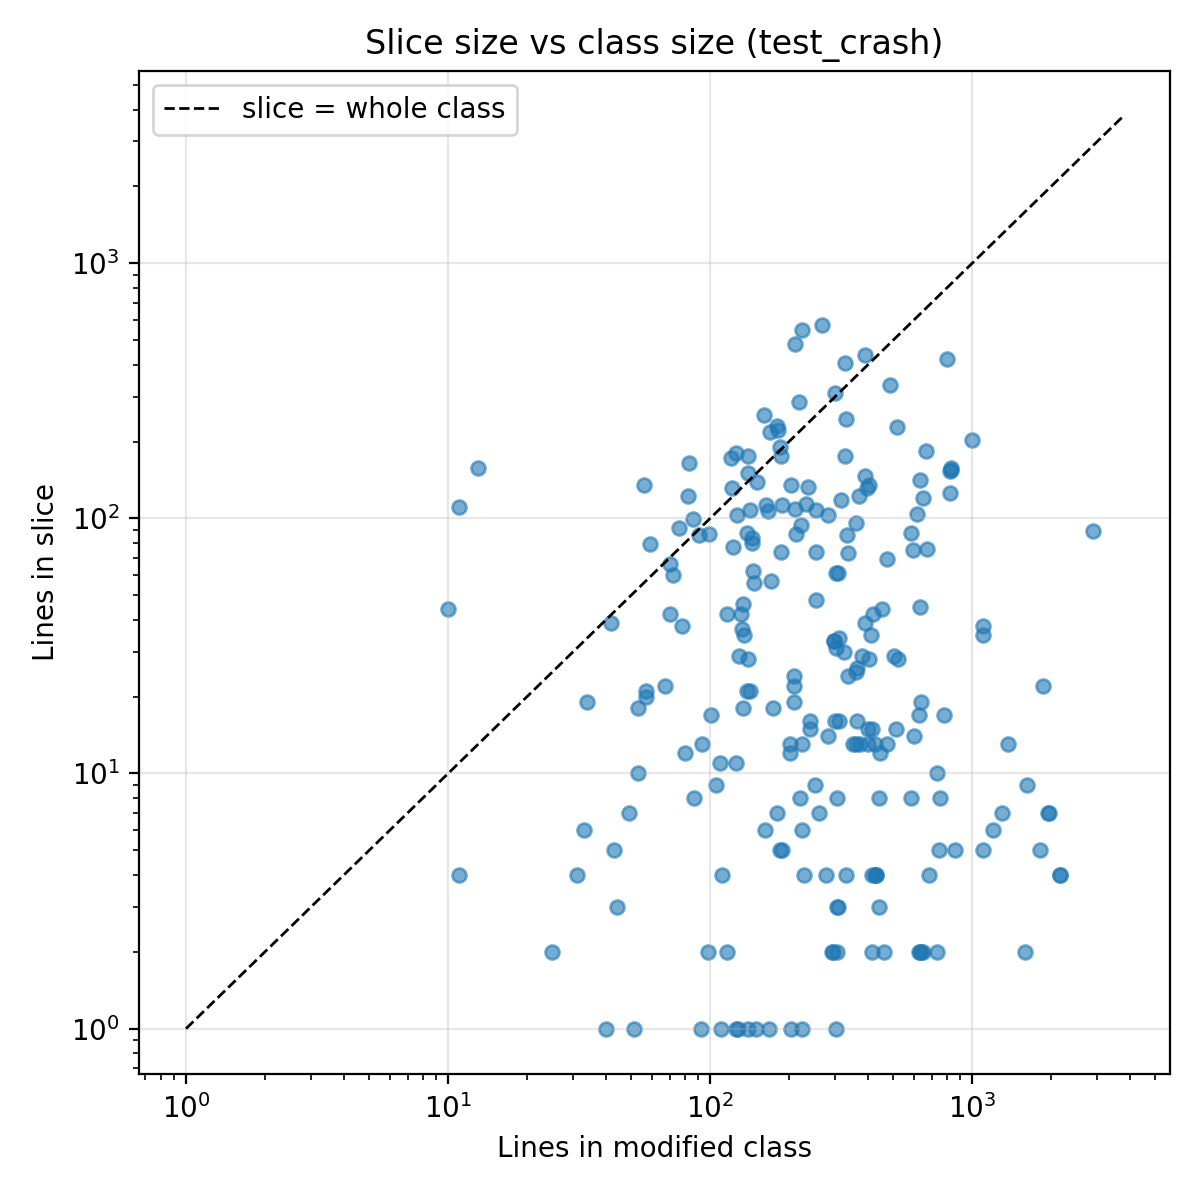
\includegraphics[width=\linewidth]{fig3_slice_vs_class}
  \caption{Figure 4}
  \Description{Scatter plot showing lines in slice versus lines in modified class under the test_crash criterion.}
  \label{fig:slice_vs_class}
\end{figure}

When we compare 78 defects which are common in succesfull runs with slice on both test\_crash and app\_deepest, the slice from the deeper application frame are much larger than the one from shallow test frame which is median of 64 against 18 with values of Holm-corrected $p = 1.09 \times 10^{-6}$ and Cliff's $\delta = 0.388$,medium. When we do same selection with respect to patched and test\_crash we get 178 defects with median slice of 56 against 23 lines with values of Holm-corrected $p = 1.05 \times 10^{-3}$; $\delta = 0.223$, small. Interestingly both patched and app\_deepest who depend of application frame have values of $p = 0.667$ with $\delta = -0.001$ which is too small to detect and matter. So the criterion which uses the test frame has the smallest slices and the criterion which uses application frame have bigger slices.

% > [I checked online and had discussion with claude for what can be used for comparision and used this , I rejected wilson interval and rank for comparision]

\subsection{Fault coverage and ground-truth anchoring}
In this section we look at the fault coverage and anchoring results.\textbf{RQ2 (Fault Coverage): To what extent do the generated slices preserve the fault-relevant root-cause lines?} From the 271 defects whose patch could be classfied only 5 of them just deleted or changed lines. Out of the rest 266 defects,We saw developers either add lines or do both(78 additive and 188 mixed). A slice cannot have a line which does not exist yet so we needed anchoring rules.The 3 of the 5 who produced slice, they are from compress and other 2 never produced a slice.  

The Fault coverage is divided into FUll,PARTIAL and None. For test\_crash fault coverage for FULL is 19.5\% and any contact is 48.7 \%. For app\_deepest fault coverage for FULL is 24.1\% and any contact is 77.2\%. For patched fault coverage for FULL is 29.4 \% and any contact is 100\% as we get the criterion line where the patch resides. Table 4.4 shows expanded results.Rule D increases the percentage of FULL coverage from 24.0\% to 38.0\% and any-contact only just from 72.8\% to 73.6\% for total runs. We saw no changes for app\_deepest and patched in any contact with Rule D from Rule C. Out of the 71 runs that change coverage,We saw 67 move from PARTIAL to FULL and 4 went from NONE to something. Also 1 defect went from 1 of 12 anchor lines to 12 of 12 anchor lines. Both Rule D and Rule C have the same effect and the miss rate drops from 51.3\% to 49.6\% for rule D so main result does not change with respect to the convention. As the result does not change alot for any contact we consider it as primary coverage and FULL as secondary state to measure.

\begin{table*}[htbp]
  \caption{Table 4.4 -- Rule coverage}
  \label{tab:rule_coverage}
  \begin{tabular}{lcccccc}
    \toprule
    Criterion & Ok Runs & FULL [C] & FULL [D] & Any-contact [C] & Any-contact [D] & NONE [C] \\
    \midrule
    test\_crash & 226 & 19.5\% & 27.0\% & 48.7\% & 50.4\% & 51.3\% \\
    app\_deepest & 79 & 24.1\% & 39.2\% & 77.2\% & 77.2\% & 22.8\% \\
    patched & 187 & 29.4\% & 50.8\% & 100\% & 100\% & 0.0\% \\
    \midrule
    \textbf{Pooled} & \textbf{492} & \textbf{24.0\%} & \textbf{38.0\%} & \textbf{72.8\%} & \textbf{73.6\%} & \textbf{27.2\%} \\
    \bottomrule
  \end{tabular}
\end{table*}

\subsection{Overhead and constraints}
In this section we look at the setup and constraints . \textbf{RQ3: What is the computational cost and scalability limit of instrumentation and dynamic trace generation?}

We have the median values of setup and instrumentation to 23 seconds and 41 seconds respectively . We saw slicing is cheap compated to them as the median time was 9 seconds(maximum 1036 seconds).Also when a trace is generated , the criterion computation is cheap compared to it as anchoring rules can be generated with same trace results.Also no completed run exceeded 22.2 million trace entries or exhausted resources below 50.3 million trace entries.
Repair context needs output that can be parsed but raw slices contain output without closing brackets or declarations which cannot be parsed.For example Math raw slices contain alot of static look up initialisations. The constraint is coverage and not the size.

\section{Discussion and future work}
The 51.3 \% of runs in test\_crash without any contact can be considered a property of dynamic slicer in general and not the tool issue of Slicer4J as in backward dynamic slicing the slicer checks the what might caused to get a wrong value in from the excuted statements and not where the fault is exactly. So if the fault does not lie in the path of execution , the slicer would never reach it. As we see for Rule C the any contact is 48.7\% and 50.4 \% for Rule D in test\_crash , so the construct is structural. We see the structural reason when checking how the defects were fixed. 98.2 \% of the defects have added atleast one line , so a dynamic dependence would not reach a statements which does not exist yet. This also explains a results for patched as even when you have a seeded criterion it only reaches FULL coverage to 29.4 \% with Rule C. For the remaining the patched line are outside the dependence of the slicer. Seeing the results we believe Slicing can be a smaller part of APR as a filter as if used for context if case of dynamic slicing it has 51.3\% chance of missing the context. But with help of localisation and stack traces it can be integrated as a context in a package.

Remaining work for the project is to run the pipeline on remaining projects from Defects4J to get full analysis. Also observe the effect of slicing as context for APR and analyse the results. Lastly an open question to APR of how much token usage can be reduced if slicing is used in APR context.


\section{Conclusion}

We evaluated Slicer4J \cite{Ahmed2021Slicer4J} for 282 Defects4J \cite{Just2014Defects4J} bugs (3 slicing criteria; 846 runs) achieving 80.1\% feasibility, test\_crash. On non-degenerate slices, dynamic slicing reduced modified classes by a median of 91.45\% to 94.74\% . In terms of Rule C: any contact coverage is 48.7\% across all feasible bugs, test\_crash and 77.2\% for bugs with an active application stack frame, app\_deepest.

Methodologically, patched criteria are circular (100.0\% any-contact by construction) and serve only as an upper-bound oracle. For Rule C, and for Rule D, sensitivity bound, any-contact coverage was steady at 72.8\% and 73.6\% respectively; FULL coverage was 24.0\% and 38.0\% respectively, and we distinguished 14 of 14 Slicer4J crashes from algorithmic limitations. Future work will include using a hybrid criterion (app\_deepest, falling back to test\_crash) and measuring reduction in LLM tokens for repair prompts.

\bibliographystyle{ACM-Reference-Format}
\bibliography{sample-base}

\end{document}
\endinput
%%
%% End of file `sigconf.tex'.
